\documentclass[aps,prx,10pt,twocolumn,floatfix,superscriptaddress,showpacs,numerical,footinbib]{revtex4-1}

\usepackage{graphicx}
\usepackage{amsmath}
\usepackage{amssymb}
\usepackage[utf8]{inputenc}
\usepackage{hyperref}
\usepackage[pdftex]{color}

\newcommand{\sgn}[1]{\mathrm{sgn} \left( #1 \right)}
\newcommand{\e}{\mathrm{e}}
\newcommand{\im}{\mathrm{i}}
\newcommand{\di}{\mathrm{d}}
\newcommand{\ket}[1]{| #1 \rangle}
\newcommand{\bra}[1]{\langle #1 |}
%\renewcommand{\thefootnote}{\fnsymbol{footnote}}

\newcommand{\noteAG}[1]{{\color{blue} [AG: #1]}}
\newcommand{\noteFP}[1]{{\color{magenta} [FP: #1]}}
\newcommand{\noteJM}[1]{{\color{red} [JM: #1]}}
\newcommand{\noteFdJ}[1]{{\color{cyan} [FdJ: #1]}}
\newcommand{\bs}[1]{{\boldsymbol{#1}}}


\begin{document}
%
\title{Interaction driven phases in the half-filled honeycomb lattice: an infinite density matrix renormalization group study}
%
\author{Good people}
\affiliation{\mbox{Max-Planck-Institut f\"ur Physik komplexer Systeme, N\"othnitzer Str.\ 38, 01187 Dresden, Germany}}
%
\date{\today}
%
\begin{abstract}
%
This is an abstract. \noteAG{There are specific commands to leave comments like this one}\noteFP{or this}\noteJM{or this}\noteFdJ{or this}
%
\end{abstract}
%
\maketitle
%

\section{Introduction}
%
The Haldane model~\cite{H88} is amazing.
%

%
Emergence of the Chern insulator state.


\section{Model and Method}
%
Method \noteAG{If we use it, we might want to define the entanglement spectrum here}\\
%
In this work we focus on spinless electrons in a honeycomb lattice with real  nearest neighbor hopping $t$ and nearest and next to nearest neighbor interactions 
$\left\lbrace V_{1},V_{2}\right\rbrace$. 
%
The Hamiltonian for this system can be written as
 %
\begin{eqnarray}
\nonumber
%
H&:=&-t\sum_{\left\langle i,j\right\rangle ,s,s'}(c^{\dagger}_{i,s}c_{j,s'}+h.c.)\\
%
\;&+&
V_{1}\sum_{\left\langle i,j\right\rangle ,s }n_{i,s}n_{j,\bar{s}}+
%
V_{2}\sum_{\left\langle \left\langle i,j\right\rangle \right\rangle ,s }n_{i,s}n_{j,s}\,
%
\label{eq:H}
%
\end{eqnarray}
%
here $c_{i,s}$ $(c^{\dagger}_{i,s})$  annihilates (creates) an electron at the $i$-th unit cell of the honeycomb lattice
in sublattice $s=A,B$ and $s\neq\bar{s}$. 
%
Each of the two triangular sublattices A and B is spanned by the basis vectors
$\bs{a}_{1}=\bs{\delta}_{2}-\bs{\delta}_{3}$ and 
$\bs{a}_{2}=\bs{\delta}_{3}-\bs{\delta}_{1}$ defined through the three nearest neighbors $\bs{\delta}_{1}=a(0,-1)$,  
$\bs{\delta}_{2}=a(\sqrt{3}/2,1/2)$ and $\bs{\delta}_{3}=a(-\sqrt{3}/2,+1/2)$ as shown in Fig.~\ref{fig:Defs}.

\begin{figure}
 %\includegraphics[width=\columnwidth]{pdf/unit_cell_small.pdf}
 \caption{Left: Hoppings and interactions of Hamiltonian \eqref{eq:H}. Right: Honeycomb lattice of $3 \times 2$ unit cells. The unit cell used for the iDMRG calculations consists of $3 \times 6$ honeycomb unit cells which yields a total circumference of 12 sites. \label{fig:Defs}}
\end{figure}
%
\begin{figure*}[tb]
 \includegraphics[scale=0.2]{Fig1.eps}
 \caption{ 
  }
  \label{fig:honeycomblattice}
\end{figure*} 
% 
\section{Phase diagram}
%
We have used the iDMRG method presented in the previous section
to find the groundstate of the half-filled graphene lattice in the presence of 
$\left\lbrace V_{1},V_{2}\right\rbrace$ interactions
%
Our results are summarised in the phase diagram presented in Fig.~\ref{fig:phase diagram}.
%
As a function of $\left\lbrace V_{1},V_{2}\right\rbrace$ we find six different ordered phases and none of them correspond to the Haldane Chern insulator.
%
In what follows we describe their corresponding charge and bond ordering patterns and analyse the different phase transitions that occur between them.
%

\begin{figure}
 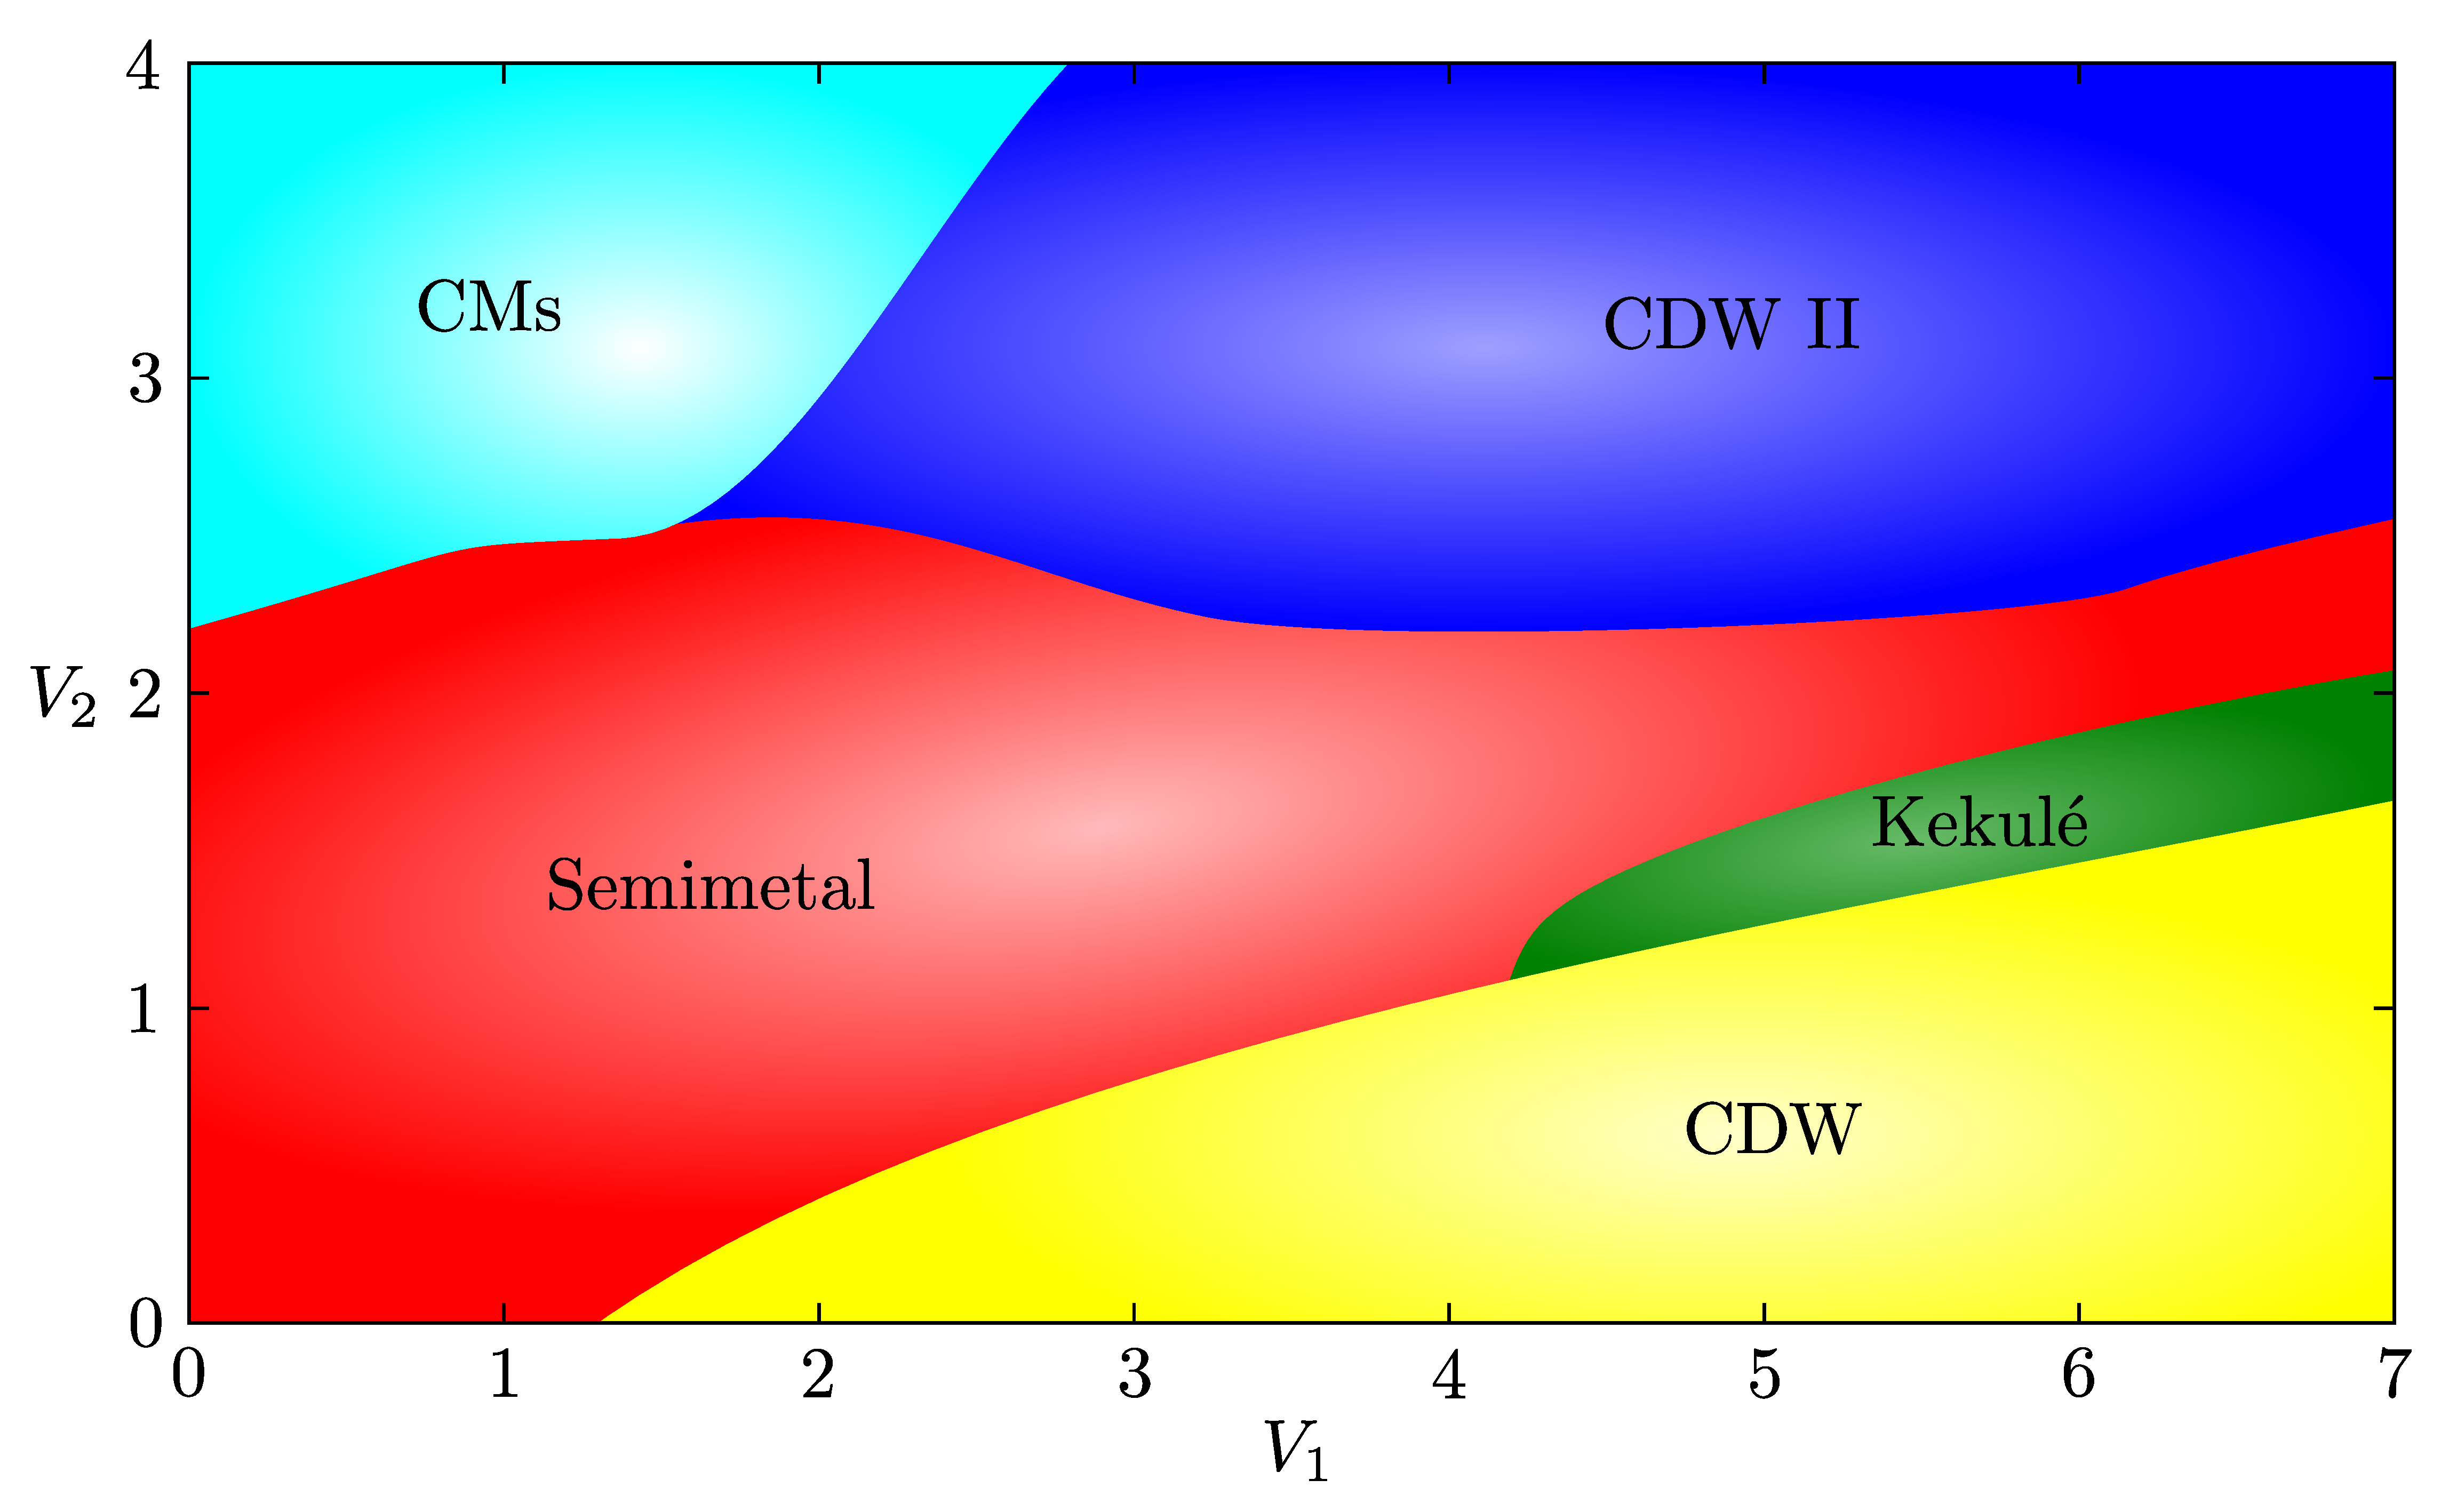
\includegraphics[width=\columnwidth]{pdf/phase_diagram.pdf}
 \caption{Phase diagram obtained with iDMRG calculations on an infinte cylinder of circumference $L=12$. \label{fig:phase diagram}}
\end{figure}

%
\subsection{Semimetal phase}
%
We start by discussing the phase diagram in the region where $\left\lbrace V_{1},V_{2}\right\rbrace < t$.
%
In this part we find that the groundstate is a semimetal phase, labelled SM in the phase diagram shown in Fig.~\ref{}.
%
This phase is characterised by a uniform renormalization of the hopping strength 
$t$ by interactions and is therefore smoothly connected to the gapless non-interacting state $V_{1}=V_{2}=0$.
%
As the latter it is a single particle gapless phase that lacks both charge and bond order and described by a low energy theory in terms of two massless Dirac cones.
%
In this latter low energy picture and within the renormalisation group approach the stability of the semimetal phase for small $\left\lbrace V_{1},V_{2}\right\rbrace$ is expected.
%
Short range interactions are irrelevant~\cite{Shankar?} and therefore they can only drive a transition to an ordered state when they have a magnitude comparable to the nearest neighbour hopping strength $t$.
%
Accordingly we find that the semimetal is stable within this region of phase space.

Within the iDMRG algorithm we have characterised the semimetal phase in three distinct ways.
%
Firstly we compute the charge and bond ground state expectation values.
%
On the one hand, at each site the charge expectation value is defined by 
%
\begin{eqnarray}
\label{eq:charge}
n_{i,s}=\left\langle c^{\dagger}_{i,s}c_{i,s}\right\rangle,  
\end{eqnarray}
%
where $s=A,B$ is the sublattice index.
%
To numerical accuracy we find that $n_{i,A}=n_{i,B}=1/2$, indicating that this phase is not charge ordered.
%

The bond ground state expectation value on the other hand is defined as
%
\begin{eqnarray}
\label{eq:charge}
t^{s,s'}_{i,j}=\left\langle c^{\dagger}_{i,s}c_{j,s'}\right\rangle,  
\end{eqnarray}
%
For $i,j$ being nearest neighbours we find a small ($10^{-?}$) asymmetry
between bonds pointing along and around the cylinder axis.
%
Such asymmetry should vanish in a perfect semimetalic phase and indeed it is severely reduced as the bond dimension $\chi$ is increased.
% 
This suggests that the explanation for the asymmetry is indeed the cylinder geometry implemented in iDMRG, that artificially differentiates bonds in its two perpendicular directions.
%

%
Moreover, we note that the semimetal phase is a critical state and thus in principle requires an infinite $\chi$ to represent the state.
%
This leads us to the second approach to characterise the semimetal phase that makes use of the its criticality.
%
For a critical phase the entanglement entropy is expected to show a logarithmic growth with the correlation length.
\noteAG{eqn needed}
%
The proportionality constant $c/3$ defines the central charge of the theory $c$. 
%
The semimetal has two Dirac cones and therefore it is expected that $c=2$. 
%
In the appendix...
\noteAG{This last paragraph can be removed if we don't need it}

%
Lastly a very accessible




%



\subsection{Charge density wave}
%
Classically, for large $V_{1}\gg t$ the energy is minimised by a charge imbalance between the two sub lattices.
%
The resulting phase, a sublattice staggered charge density wave state (CDW), has a two site unit cell that is characterised by the order parameter
%
\begin{equation}
\label{eq:CDW}
%
M=\left\langle n_{A} \right\rangle-\left\langle n_{B}\right\rangle
%
\end{equation}
%
where $n_{A}$ and $n_{B}$ are the density of electrons in the $A$ and $B$ sublattice sites of the two site unit cell respectively.
%


\subsection{Charge modulated phase}
%

\subsection{Kekulé}
%

\subsection{Twelve site charge density wave}
%

\subsection{Twelve site charge density wave II}
%

\section{Phase transitons}
%
some phase transitions?

\begin{figure}
 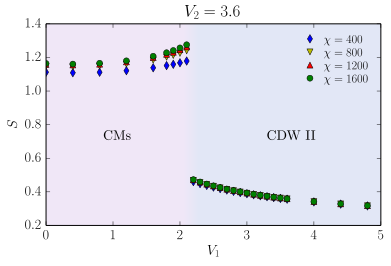
\includegraphics[width=\columnwidth]{{pdf/plot_cut_V2_3.6}.pdf}
 \caption{Entanglement entropy at $V_2=3.6$. \label{fig:cut_V2_3.6}}
\end{figure}

\begin{figure}
 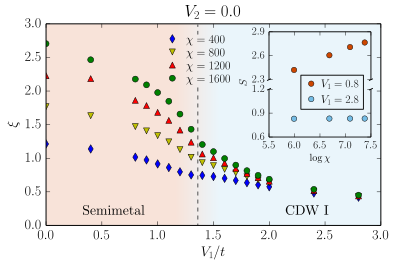
\includegraphics[width=\columnwidth]{{pdf/plot_cut_V2_0}.pdf}
 \caption{Correlation length at $V_2=0$. \label{fig:cut_V2_0}}
\end{figure}

\begin{figure}
 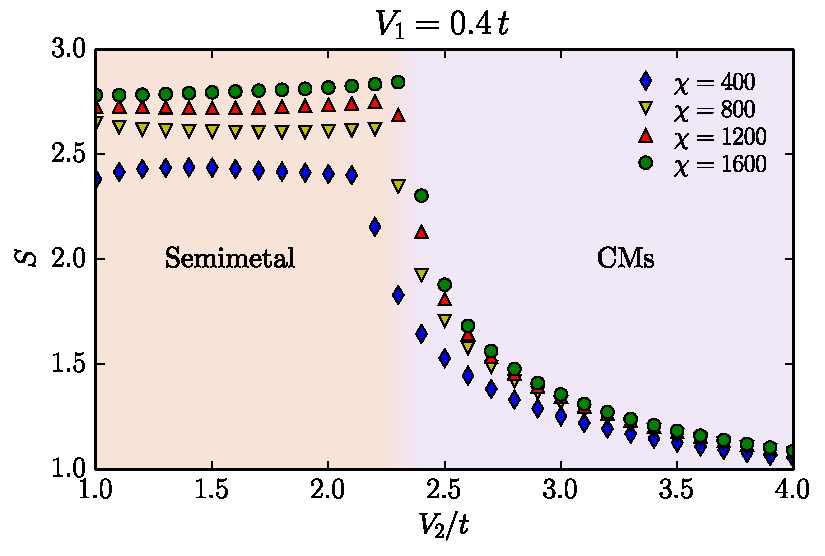
\includegraphics[width=\columnwidth]{{pdf/plot_cut_V1_0.4}.pdf}
 \caption{Entanglement entropy at $V_1=0.4$. \label{fig:cut_V1_0.4}}
\end{figure}

\begin{figure}
 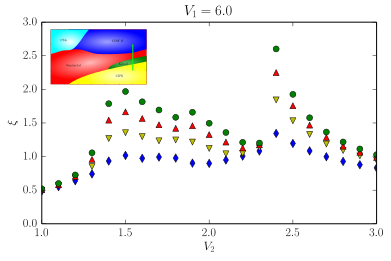
\includegraphics[width=\columnwidth]{{pdf/plot_cut_V1_6}.pdf}
 \caption{Correlation length at $V_1=6$. \label{fig:cut_V1_6}}
\end{figure}



%
\section{Discussion and Conclusions}
%
awesome conclusions

\bibliography{CI_iDMRG.bib}


\end{document}